\begin{problem}{여우 사인}{standard input}{standard output}

도주는 동물을 좋아한다. 그중에서도 여우를 정말 좋아한다! 어느 날, 힐링을 위해 여우 사진을 검색하던 도주는 ``여우 사인''이라는 손 모양을 발견했다.

\begin{center}
  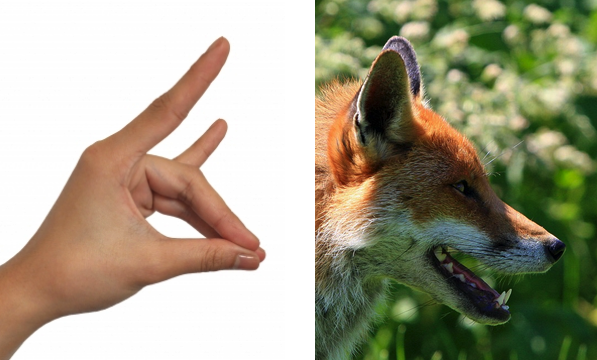
\includegraphics[width=0.6\textwidth]{fox-sign.png}
\end{center}

여우 사인은 엄지손가락, 중지, 약지의 끝을 맞닿게 하고 검지와 새끼손가락은 곧게 펴서 여우의 얼굴과 두 귀를 표현한 손 모양이다.

도주는 자신의 여우 사랑을 널리 알리기 위해 때때로 이 손 모양을 하고 귀여운 척을 하기로 했다. 도주의 손 모양이 주어질 때, 그것을 여우 사인이라고 할 수 있는지 판별해 보자. 손 모양을 판별할 때는 손가락이 곧게 펴져 있는지 구부러져 있는지, 손가락의 어느 부분이 닿아 있는지 등의 사소한 것은 신경 쓰지 않기로 한다.

\InputFile
첫 번째 줄에 서로 닿아 있는 손가락 쌍의 개수 $N$($1 \le N \le 10$)이 주어진다.

두 번째 줄부터 $N$개의 줄에 걸쳐 서로 닿아 있는 두 손가락을 의미하는 $1$ 이상 $5$ 이하의 숫자 두 개가 공백으로 구분되어 주어진다. $1$은 엄지손가락, $2$는 검지, $3$은 중지, $4$는 약지, $5$는 새끼손가락을 의미한다.

입력 순서가 다른 것을 포함하여 같은 쌍이 여러 번 주어지거나 한 손가락만으로 이루어진 쌍이 주어지는 경우는 없다.

\OutputFile
첫 번째 줄에 도주의 손 모양을 여우 사인이라고 할 수 있으면 \texttt{Wa-pa-pa-pa-pa-pa-pow!}를, 그렇지 않으면 \texttt{Woof-meow-tweet-squeek}을 출력한다.

\Example

\begin{example}
\exmp{3
1 3
4 3
1 4}{Wa-pa-pa-pa-pa-pa-pow!}%
\exmp{5
1 3
3 4
4 1
1 5
5 4}{Woof-meow-tweet-squeek}%
\end{example}

\Notes
첫 번째 예시는 엄지손가락과 중지, 약지와 중지, 엄지손가락과 약지가 서로 닿아 있고 검지와 새끼손가락은 다른 손가락과 닿아 있지 않으므로 여우 사인이라고 할 수 있다.

두 번째 예시는 검지만 펴고 다른 손가락은 접은 손 모양이다.

\end{problem}
